\documentclass[12pt]{article}
\usepackage[a4paper, margin=.30in]{geometry}
\usepackage{graphicx ,
            wrapfig,
            xcolor, 
            enumerate,
            amsmath,fontenc, mhchem,makecell, mhchem,tcolorbox,tikz,fancyhdr
            }

\newcommand\headerMe[2]{\noindent{}#1\hfill#2}
\renewcommand{\thesection}{\Roman{section}}
\title{LES ondes électromagnétiques leçon}
\author{Zakaria HAOUZAN}
\date{\today}

\pagestyle{fancy}
\fancyhf{}
\rhead{2022/2023}
\lhead{Pr: Zakaria HAOUZAN}
\chead{Physique Chimie}
\rfoot{lycée :  skhor rhamna}
\cfoot {Page \thepage}


\begin{document}
% headers --------------
\headerMe{Matière : Physique-Chimie}{Professeur : Zakaria HAOUZAN}\\
\headerMe{Unité :Sens d'évolution d'un\\système chimique  }{Établissement : Lycée SKHOR qualifiant}\\
\headerMe{Niveau : 2BAC-SM-PC}{Heure : 2H}\\

% ------Content ________


\begin{center}

    \Large{Leçon $N^{\circ} 6 $: \color{red}Sens d'évolution d'un système chimique }
\end{center}
\section{Quotient de la réaction :}
\subsection{Définition (Rappel) :}
Le quotient de la réaction est une grandeur qui caractérise un système chimique dans un état donné.

Sa valeur nous renseigne sur l'évolution du système étudié.
On considère la transformation chimique modélisée par la réaction suivante:

$$\ce{\alpha.A_{(aq)} + \beta.B_{(aq)} <=> \gamma.C_{(aq)} + \delta.D_{(aq)}}$$
Le quotient de cette réaction  s'écrit : $$Q_r = \frac{[C]^{\gamma}.[D]^{\delta}}{[A]^{\alpha}.[B]^{\beta}}$$

$Q_r$ est une grandeur sans Unité.

[A],[B],[C] et [D] concentrations molaires des espéces chimiques exprimées en mol/L.
\begin{tcolorbox}
Seules sont représentées les espèces dissoutes en solution, ce qui exclut les solides, les précipités, les
gaz non dissous et le solvant souvent l'eau. Qr est sans unité.
A l'équilibre, Qr,éq = K (constante d'équilibre).
\end{tcolorbox}

\section{Critère d'évolution spontanée : }

Une évolution est spontanée si elle se produit sans intervention extérieure.
Au cours du temps, la valeur du quotient de réaction Qr tend vers la constante d'équilibre K.
Les trois situations qui peuvent être envisagées : $Qr,i < K$ , $Qr,i > K$ ou $Qr,i = K$ :

\textbf{\underline{1. Qr,i = K}}

Le système chimique est à l'équilibre. La réaction se fait dans les 2 sens mais le mélange n'évolue
pas. Les concentrations des espèces chimiques ne varient plus, Qr reste constant.

\textbf{\underline{2. $Qr,i < K$}}

$$\ce{\alpha.A_{(aq)} + \beta.B_{(aq)} <=> \gamma.C_{(aq)} + \delta.D_{(aq)}}$$
$$Q_r = \frac{[C]^{\gamma}.[D]^{\delta}}{[A]^{\alpha}.[B]^{\beta}}$$

Si $Qr,i < K$, cela signifie que le système va évoluer de façon à ce que Qr augmente pour tendre vers K.
Il faut donc créer des espèces C et D, et consommer A et B, le système va donc évoluer dans le sens
direct de l'équation de la réaction.
Cette évolution s'arrêtera lorsque le quotient de la réaction atteindra la valeur de la constante
d'équilibre K.

\textbf{\underline{3. $Qr,i > K$}}

Si $Qr,i > K$, cela signifie que le système va évoluer de façon à ce que Qr diminue pour tendre vers K .
Il faut donc créer des espèces A et B, et consommer C et D, le système va donc évoluer dans le sens
inverse de l'équation de la réaction. Cette évolution s'arrêtera lorsque le quotient de la réaction
atteindra la valeur de la constante d'équilibre K.

\textbf{\underline{4. Diagramme de critère d'évolution :}}
\begin{center}
	\definecolor{costumColor}{rgb}{0,0.6,0.5}
\begin{tikzpicture}

\draw[line width=0.1cm, blue] (0,0) node[above] {$Qr,i<K$}-- (5,0) ;
	\draw[line width=0.1cm ,costumColor, ->] (5,0) -- (10,0) node[above] {$Qr,i>K$}node[right] {Qr,i} ;
	\draw[line width=0.1cm, magenta] (5,-5pt) node[below]  {Qr,i = K} node[above=5pt] {équilibre}-- (5,5pt);

	\draw[blue, ->, thick] (0.5,-0.5) node[below] {évolution dans le sens direct} -- (4,-0.5);
	\draw[costumColor, <-] (6,-0.5) -- (9.5,-0.5)node[below] {évolution dans le sens inverse} ;
\end{tikzpicture}
\end{center}


\section{Application du critère d'évolution spontanée : }
\subsection{Réaction acido-basique :}
\section*{Exercice : On mélange les solutions suivantes :}

\begin{itemize}
	\item  $V_1 = 5,0 mL$ d'une solution d'acide méthanoïque de concentration $C_1 = 3,0.10^{- 2} mol.L^{-1}.$
		
	\item $V_2 = 10,0 mL$ d'une solution de chlorure d'ammonium de concentration $C_2 = 4,0.10^{-2} mol.L^{-1}$

	\item $V_3 = 5,0 mL$ d'une solution de méthanoate de sodium de concentration $C_3 = 6,0.10^{- 2} mol.L^{-1}$.

\item $V_4 = 10,0 mL$ d'une solution d'ammoniaque de concentration $C_4 = 8.10^{- 2} mol.L^{-1}$

\item[a)] Calculer le quotient de réaction initial en considérant l'acide méthanoïque comme un réactif.
\item[b)] Préciser le sens d'évolution spontanée de ce système chimique.
\end{itemize}

Données : couple $HCOOH / HCOO^-$ : $pKA_1 = 3,8$ et couple $NH_4^+/NH_3$ : $pKA_2 = 9,2$

c/c : D'après le critère d'évolution spontanée, le système chimique va évoluer dans le sens direct de
l'équation de la réaction.

\subsection{Réaction d'oxydo-réduction :}

\section*{Exercice : On mélange les espèces suivantes :}

\begin{itemize}

	\item  $V_1 = 20 mL$ d'une solution de chlorure de fer (III) de concentration $C_1 = 3,0.10^{- 2} mol.L^{-1}.$

	\item $V_2 = 20 mL$ d'une solution de sulfate de fer (II) de concentration $C_2 = 2,0.10^{ -2} mol.L^{-1}.$

	\item $V_3 = 10 mL$ d'une solution de sulfate de cuivre (II) de concentration $C_3 = 1,0.10^{-1} mol.L^{-1}$

	\item $10 g$ de poudre de cuivre.
	\item \textbf{Données :} couples  $Fe^{3+} / Fe^{2+}$ et $Cu^{2+}/ Cu$
	\item[a) ] Ecrire l'équation de la réaction susceptible de se produire entre le cuivre et les ions $Fe^{3+}$.

	\item[b)] Calculer le quotient de réaction initial associé à cette équation.
	\item[c)] Déterminer le sens d'évolution spontanée de la réaction où $K = 3,8.10^{ 40}$

\end{itemize}
c/c : Par conséquent, d'après le critère d'évolution spontanée, le système chimique va évoluer dans le sens
direct de l'équation de la réaction.


%\begin{figure}[h!]
	%\begin{center}
	%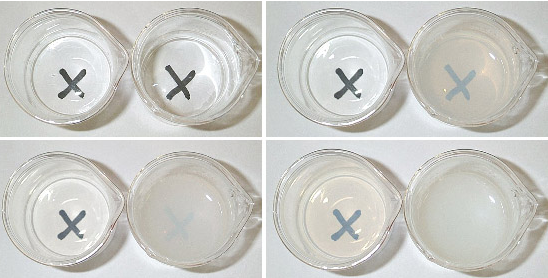
\includegraphics[width=0.5\textwidth]{./img/TRLconcentration.png}
%\end{center}
%\vspace{-1cm}
%\end{figure}



%\begin{wrapfigure}[10]{r}{0.5\textwidth}
%    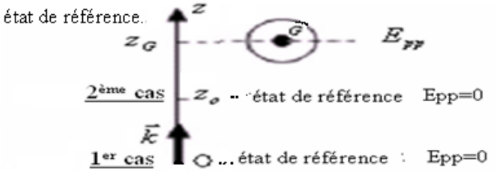
\includegraphics[width=0.5\textwidth]{./img/img00.png}
%\end{wrapfigure}


%\begin{center}
   %\begin{tabular}{|c|c|c|}
      %\hline
      %Indicateur coloré & Couleur de l’espèce acide & Couleur de l’espèce base\\\hline
      %BBT               & Jaune                     & Bleue\\\hline
      %Hélianthine       &Rose                       & Jaune\\\hline
      %Phénolphtaléine   & inclore                   & rose \\\hline
   %\end{tabular}
%\end{center}

\end{document}

